\documentclass[11pt, a4paper]{article}
\usepackage[a4paper, top=20mm, left=20mm, right=20mm, bottom=20mm]{geometry}
\usepackage{hyperref}
\usepackage[sf]{titlesec}
\usepackage{listings}
\usepackage{graphicx}

\hypersetup{hidelinks = true}

\begin{document}
{\fontfamily{cmss}\selectfont

\title{\vspace{-20mm}CMPUT 291 - Mini Project 1 Design Document}
\date{}
\maketitle
\vspace{-20mm}
\section{Overview}\label{OV}
The following python application is used to connect to an existing SQLite3 database storing enterprise data. The application is run through the terminal, and is operated with simple command line inputs. For informatino on connecting to a database and running the application, see \emph{\nameref{UG}}.

Users with valid login credentials will be provided access to various functions to interact, view, and update the data stored in the database. Depedning on their user type (determined by the databes) the functionalities include: \emph{Register a birth, Register a marriage, Renew a vehicle registration, Process a bill of sale, Process a payment, Get a driver abstract, Issue a ticket, Find a car owner}. For speceifics on these functions and thei operations, see \emph{\nameref{SD}}.

\subsection{User Guide}\label{UG}
To launch the application, run the following command from the directory holding the source code:
\begin{centering}
\begin{lstlisting}[language=Python]
	$ python3 db.py
\end{lstlisting}
\end{centering}
To connect to a database, enter the path to the database when prompted:
\begin{lstlisting}[language=Python]
	Enter path of database: path/to/database.db
\end{lstlisting}
If the database connection is successfuly established, the user will be prompted to enter their username and password:
\begin{lstlisting}[language=Python]		
	Username: admin123
	Password: pwd12345
\end{lstlisting}
Depending in the user type (agent or officer), numerical options will appear on screen. Enter the number of the task you wish to perform, and follow the on-screen instructions. For further information regarding the options, see \emph{\nameref{SD}}


\subsection{Flow Diagram}
\begin{center}
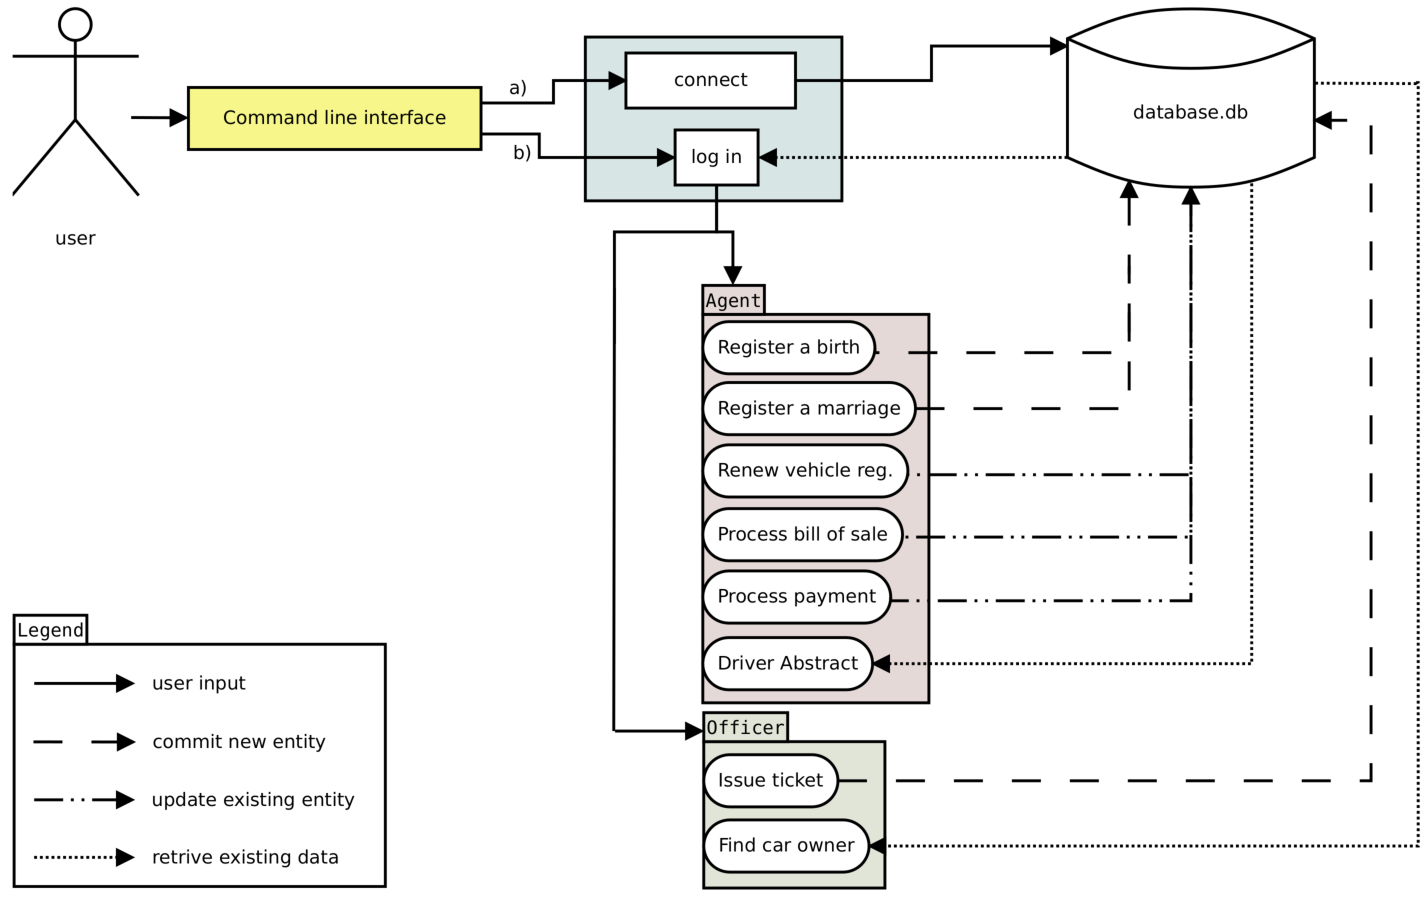
\includegraphics[width=0.5\textwidth]{Diagram1.pdf}
\end{center}

\newpage
\section{Software Design}\label{SD}
Describe the responsibility and interface of each primary function:
\begin{itemize}
\item Register a birth
\item Register a marriage
\item Renew a vehicle registration
\item Process a bill of sale
\item Process a payment
\item Get a driver abstract
\item Issue a ticket
\item Find a car owner
\end{itemize}

\section{Testing Strategy}\label{TS}
The testing strategy discusses your general strategy for testing, with the scenarios being tested, the coverage of your test cases and (if applicable) some statistics on the number of bugs found and the nature of those bugs. 

\section{Group Break-down Strategy}\label{GS}
The group work strategy must list the break-down of the work items among partners, both the time spent (an estimate) and the progress made by each partner, and your method of coordination to keep the project on track. The design document should also include a documentation of any decision you have made which is not in the project specification or any coding you have done beyond or different from what is required.

\end{document}

 
